% Owner: Lynn. Supporting material for sections 5 and 6; appendices don't count towards the 10 pages.
\appendix
\section{Implementation details}\label{app:implementation}

\paragraph{Version constraints.} MinIO stopped publishing free official container images in 2025, so we
pin the last free build archived by Bitnami. Airflow follows the course lab's major version (2.x) with
the lighter LocalExecutor, which needs no Redis or Celery workers on a single machine.

% The dashboard is a page tall, so it sits here; section 6 refers to it.
\begin{figure}[p]
  \centering
  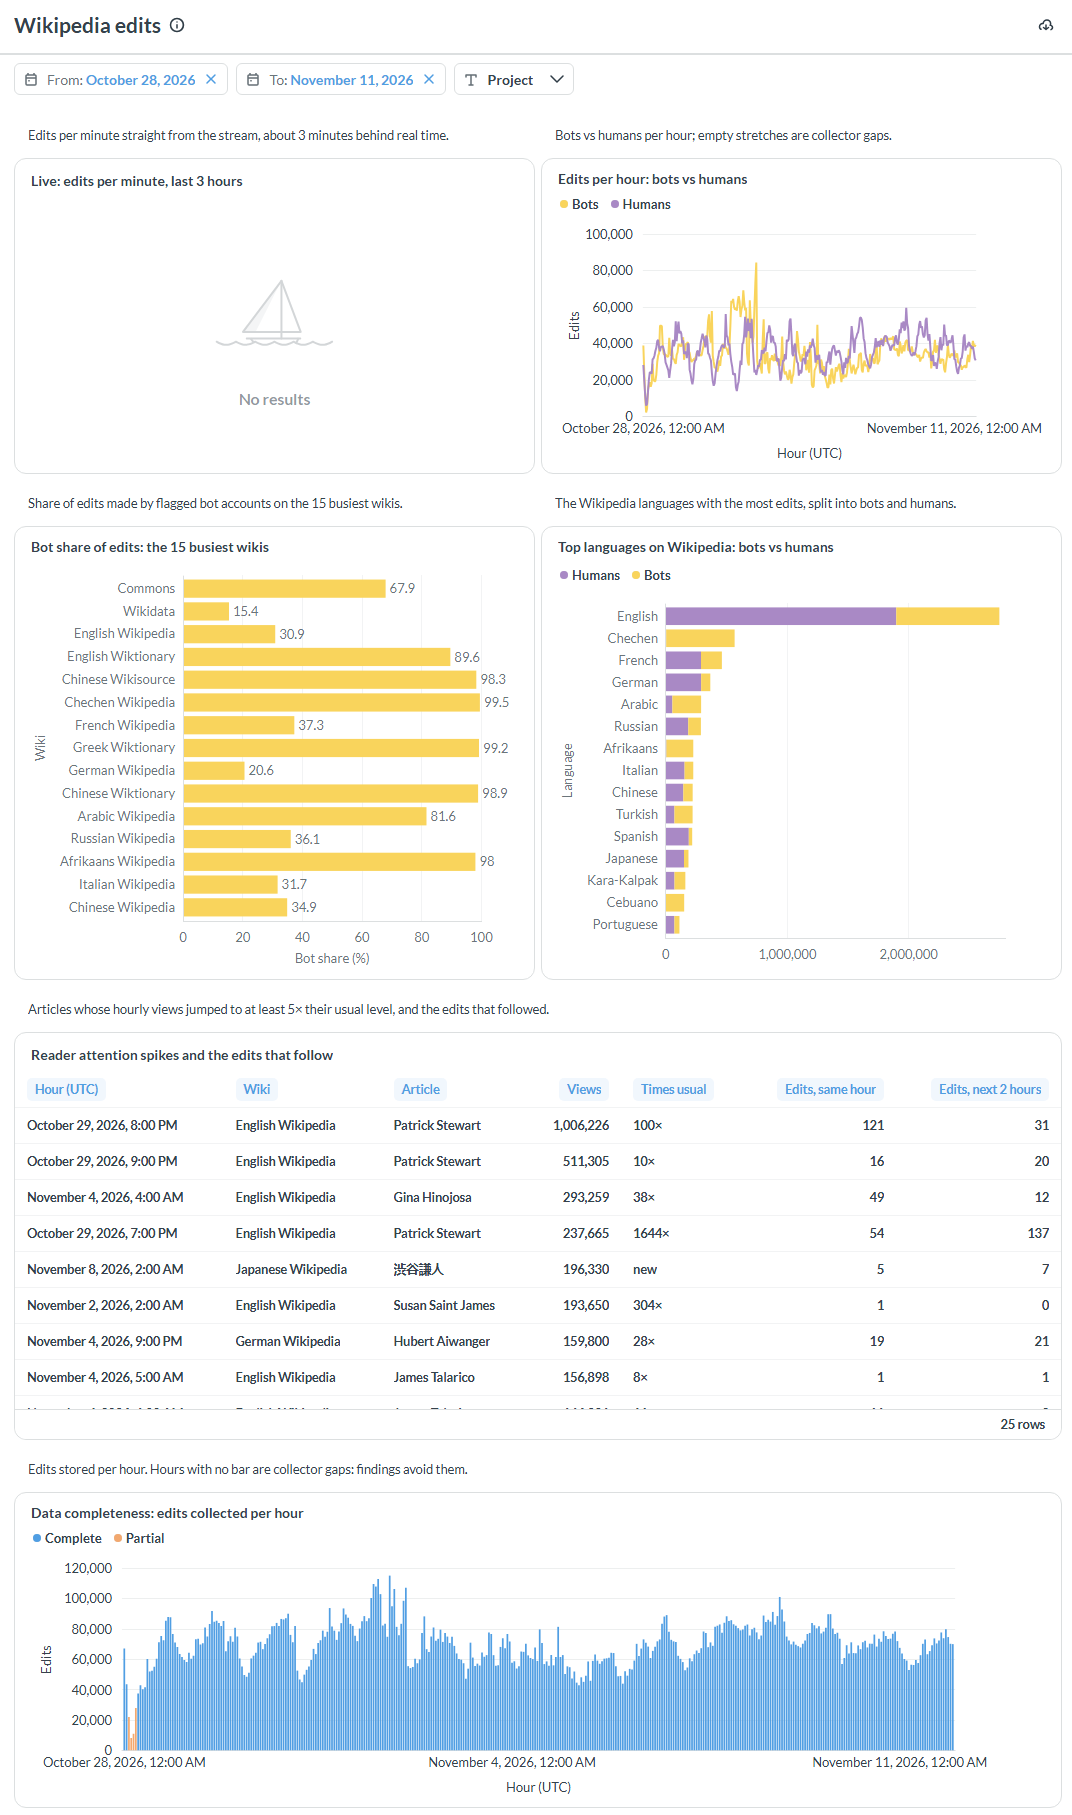
\includegraphics[height=0.9\textheight]{06_dashboard.png}
  \caption{The \emph{Wikipedia edits} dashboard over the analysis window, 28 Oct -- 11 Nov 2026 (UTC),
    taken on 23 Nov. The live tile is empty because the collector was stopped after the window closed.}
  \label{fig:dashboard}
\end{figure}

\begin{table}[!htbp]
  \centering\small
  \begin{tabular}{lcll}
    \toprule
    Topic & Partitions & Written by & Read by (consumer group) \\
    \midrule
    \texttt{wiki.raw}          & 3 & producer  & raw sink, processor \\
    \texttt{edits.bot}, \texttt{edits.human} & 3 each & processor & clean sinks $\times$2 \\
    \texttt{edits.per\_minute} & 1 & processor & live-stats \\
    \texttt{wiki.deadletter}   & 1 & processor & inspected by hand \\
    \bottomrule
  \end{tabular}
  \caption{Kafka topics and consumer groups.}
  \label{tab:topics}
\end{table}

\begin{figure}[!htbp]
  \centering
  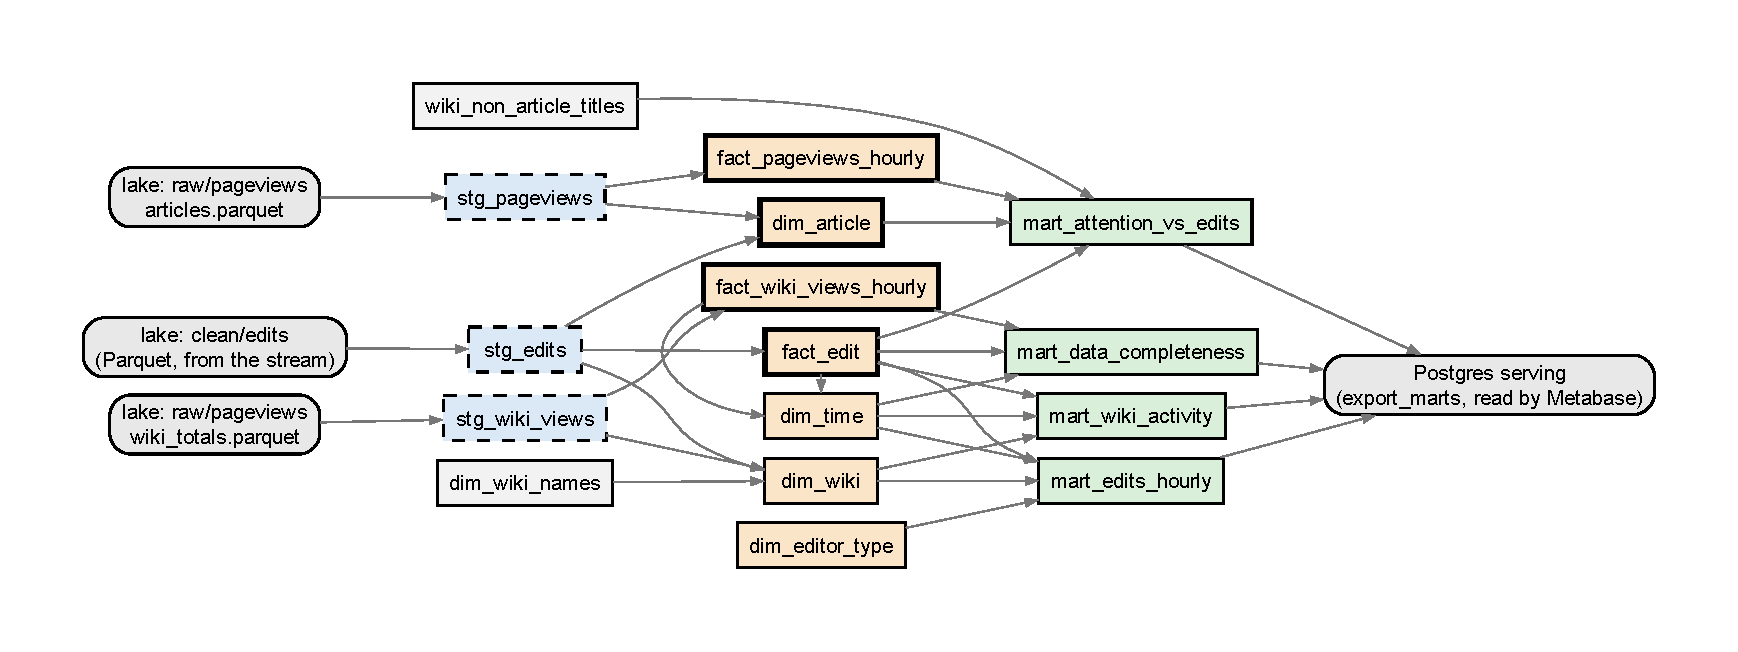
\includegraphics[width=\linewidth]{lineage.pdf}
  \caption{dbt lineage, generated from dbt's manifest (\texttt{scripts/lineage\_figure.py}). Dashed:
    views; bold: incremental tables; plain: tables (and the \texttt{dim\_wiki\_names} seed).}
  \label{fig:lineage}
\end{figure}

\begin{table}[!htbp]
  \centering\small
  \begin{tabularx}{\linewidth}{l>{\raggedright\arraybackslash}X>{\raggedright\arraybackslash}X}
    \toprule
    Date & What happened & Fix \\
    \midrule
    27 Oct & Resuming with a \texttt{Last-Event-ID} header was silently ignored; replays ended with
      almost nothing & Replay by time with \texttt{?since=} \\
    3 Nov & Wikimedia drops long connections every few minutes; a 16-hour replay restarted from its
      beginning each time and looped for two hours & Save how far a replay got and resume there \\
    5 Nov & After 9 hours asleep, the replay filled the sinks' buffers ($\approx$1\,GB) and dbt was
      killed for lack of memory & Sinks also flush every 50,000 events \\
    7 Nov & A replay sends one data centre's topic up to now, then the other's. Judging the end of a gap
      across both ended three replays with 0--202 events, leaving holes on 3 and 6 Nov & Track each
      topic separately; the holes were replayed (1,459,669 events) \\
    7 Nov & Events recovered more than a day late never reached the warehouse, and the status check
      still reported no gaps & Reload the last three days; count gaps on the deduplicated clean zone and
      flag half-empty hours \\
    8--10 Nov & Windows put the laptop into standby with the screen off although sleep was disabled
      (longest: 5\,h 47\,min) & Replayed after waking (511,225 events for the longest) \\
    8--10 Nov & Four warehouse runs failed a relationship test (fact rows whose article was missing
      from \texttt{dim\_article}) & The gate kept the last good data and the next run passed. Most likely
      cause: both models read the live clean zone, so files written between them reach
      \texttt{fact\_edit} but not \texttt{dim\_article}; reading only hours before the run's start would
      remove it \\
    9--12 Nov & Hourly rebuilds grew Docker's disk file to 351\,GB (46\,GB in use), and its file system
      recorded errors; some writes to the warehouse file were lost & Checked every lake file against its
      event count (all intact), repaired and shrank the disk, rebuilt the warehouse from the lake \\
    \bottomrule
  \end{tabularx}
  \caption{Collector and warehouse incidents during the window.}
  \label{tab:incidents}
\end{table}
